\documentclass[UTF8,12pt]{article}
\usepackage{ctex}
\usepackage{indentfirst}
\usepackage{color}
\usepackage{hyperref}
\usepackage{graphicx}
\usepackage{subfigure}
\usepackage{pdfpages}
\usepackage{listings}
\usepackage{afterpage}

\newcommand\myemptypage{
    \null
    \thispagestyle{empty}
    \addtocounter{page}{-1}
    \newpage
}

\hypersetup{
    hidelinks,
	colorlinks=true,
	allcolors=black,
	pdfstartview=Fit,
	breaklinks=true
}

\definecolor{dkgreen}{rgb}{0,0.6,0}
\definecolor{gray}{rgb}{0.5,0.5,0.5}
\definecolor{mauve}{rgb}{0.58,0,0.82}

\lstset{ %
  language=Octave,                % the language of the code
  basicstyle=\footnotesize,           % the size of the fonts that are used for the code
  numbers=left,                   % where to put the line-numbers
  numberstyle=\tiny\color{gray},  % the style that is used for the line-numbers
  stepnumber=2,                   % the step between two line-numbers. If it's 1, each line 
                                  % will be numbered
  numbersep=5pt,                  % how far the line-numbers are from the code
  backgroundcolor=\color{white},      % choose the background color. You must add \usepackage{color}
  showspaces=false,               % show spaces adding particular underscores
  showstringspaces=false,         % underline spaces within strings
  showtabs=false,                 % show tabs within strings adding particular underscores
  frame=single,                   % adds a frame around the code
  rulecolor=\color{black},        % if not set, the frame-color may be changed on line-breaks within not-black text (e.g. commens (green here))
  tabsize=2,                      % sets default tabsize to 2 spaces
  captionpos=b,                   % sets the caption-position to bottom
  breaklines=true,                % sets automatic line breaking
  breakatwhitespace=false,        % sets if automatic breaks should only happen at whitespace
  title=\lstname,                   % show the filename of files included with \lstinputlisting;
                                  % also try caption instead of title
  keywordstyle=\color{blue},          % keyword style
  commentstyle=\color{dkgreen},       % comment style
  stringstyle=\color{mauve},         % string literal style
  escapeinside={\%*}{*)},            % if you want to add LaTeX within your code
  morekeywords={*,...}               % if you want to add more keywords to the set
}


\setlength{\parindent}{2em}

\begin{document}

\begin{titlepage}
    \includepdf[pages={1}]{cover.pdf}
\end{titlepage}

\myemptypage

\begin{center}
    \tableofcontents
\end{center}
\newpage

\section{预习任务}
\begin{itemize}
    \item 对界面的操作进行定义,实现各个界面的基本功能
    \item 配置android网络
\end{itemize}

\section{预习内容}

\subsection{界面操作实现}
\subsubsection{启动界面}
用户点击软件图标之后,先进入启动页面,展示图标和软件名称,然后跳转到登录界面,右上角有一个跳过按钮,点击之后直接跳转到主界面。

实现activity为SplashActivity,点击“跳过”时,直接跳转到登录页面,具体如下:

\begin{lstlisting}[frame=shadowbox]
    public class SplashActivity extends AppCompatActivity {

    private Handler mHandler = new Handler();
    private Button mBtnSkip;

    private Runnable mRunnableToMain = new Runnable() {
        @Override
        public void run() {
            toLoginActivity();
        }
    };

    private void toLoginActivity() {
        Intent intent = new Intent(this, LoginActivity.class);
        startActivity(intent);
        finish();
    }

    @Override
    protected void onCreate(Bundle savedInstanceState) {
        super.onCreate(savedInstanceState);
        setContentView(R.layout.activity_splash);

        mBtnSkip = (Button) findViewById(R.id.id_btn_skip);
        mHandler.postDelayed(mRunnableToMain, 3000);

        mBtnSkip.setOnClickListener(new View.OnClickListener() {
            @Override
            public void onClick(View view) {
                mHandler.removeCallbacks(mRunnableToMain);
                toLoginActivity();
            }
        });

    }
}

\end{lstlisting}

\subsubsection{登录/注册界面}
用户经过启动页面之后,进入登录页面,用户根据自身需求选择:跳转到注册界面,或直接输入账号密码进行登录。

若跳转到注册界面,用户输入账号密码,点击注册按钮,将账号密码发送到服务器,服务器返回注册成功或失败的信息,若成功,则跳转到登录界面,若失败,则提示用户注册失败。

若直接登录,则用户输入账号密码,点击登录按钮,将账号密码发送到服务器,服务器返回登录成功或失败的信息,若成功,则跳转到主界面,若失败,则提示用户登录失败。

具体的流程图如下:

\begin{figure}[htbp]
    \centering
    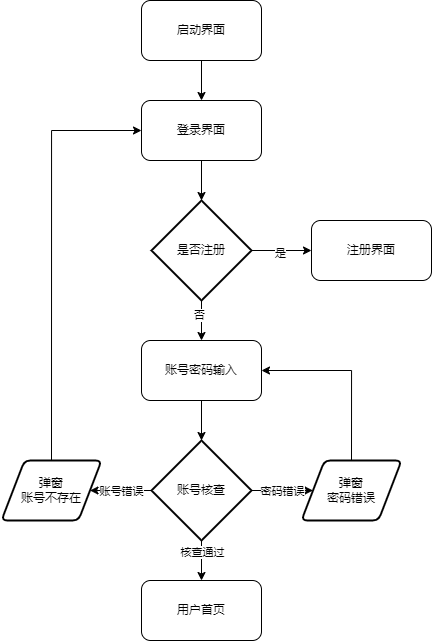
\includegraphics[width=0.8\textwidth]{imgs/1.png}
    \caption{登录/注册流程图}
\end{figure}

\newpage

在应用端只负责提交数据,不负责验证数据,验证数据的工作交给服务器端,也就是说应用端只需要提取输入框的输入即可,返回的提示用toast实现,具体代码如下:

\begin{lstlisting}[frame=shadowbox]
    public String requestDataByPost(String urlString) {
        String result = null;
        try {
            URL url = new URL(urlString);
            HttpURLConnection connection = (HttpURLConnection) url.openConnection();
            connection.setConnectTimeout(30000);
            connection.setRequestMethod("POST");

            // 设置运行输入,输出:
            connection.setDoOutput(true);
            connection.setDoInput(true);
            // Post方式不能缓存,需手动设置为false
            connection.setUseCaches(false);
            connection.connect();

            // 我们请求的数据:
            String data = "uid=" + URLEncoder.encode(uid, "UTF-8")
                    + "&upsw=" + URLEncoder.encode(upsw, "UTF-8");
            // 获取输出流
            OutputStream out = connection.getOutputStream();
            out.write(data.getBytes());
            out.flush();
            out.close();

            int responseCode = connection.getResponseCode();
            if (responseCode == HttpURLConnection.HTTP_OK) {
                InputStream inputStream = connection.getInputStream();
                result = NetUtil.streamToString(inputStream);

                user = new Gson().fromJson(result,User.class);


            } else {
                String responseMessage = connection.getResponseMessage();

            }


            connection.disconnect();
            return result;
        } catch (MalformedURLException e) {
            e.printStackTrace();
        } catch (IOException e) {
            e.printStackTrace();
        }
        return null;
    }
\end{lstlisting}

注册与登录类似,唯一不同的是请求的数据不同,注册需要提交的数据有uid,upsw,uname,而登录只需要提交uid,upsw即可。

\begin{lstlisting}[frame=shadowbox]
    String data ="uname=" + URLEncoder.encode(uname, "UTF-8") +  "&uid=" + URLEncoder.encode(uid, "UTF-8")
    + "&upsw=" + URLEncoder.encode(upsw, "UTF-8");
\end{lstlisting}

\subsection{配置android网络}
android 和web 服务器的数据交互,涉及到android 的网络相关操作,可以选择使用第三方库或者自己编写简单的代码实现。我采用了自己编写代码,并抽取到工具类NetUtil中。

\subsubsection{配置baseurl}
首先配置类Config,里面存储了访问服务器用的url中基础的部分,本实践采用了主机作服务器,其中由于主机连接WLAN,而非有线的Ethernet,因此ip地址会变化;对于实际的工程来说,服务器的ip应当是固定的,不存在以上问题。

\begin{lstlisting}[frame=shadowbox]
    public class Config {
        public static String baseUrl ="http://100.67.123.30:8080/PalmHospitalService_war_exploded/";
    }
\end{lstlisting}

这样在其他类中,只需要将url加上这一部分,修改代码很方便。

\subsubsection{编写工具类NetUtil}
接着编写工具类NetUtil:由于数据量不大,我们都采用Get 的请求方式,将参数添加在url 末尾。编写函数requestDataByGet:参数url,进行HttpURLConnection 的相关设置,获取请求的返回码,判断是否成功等等

\begin{lstlisting}[frame=shadowbox]
    package com.example.palmhospital.utils;

    import android.util.Log;

    import java.io.ByteArrayOutputStream;
    import java.io.IOException;
    import java.io.InputStream;
    import java.net.HttpURLConnection;
    import java.net.MalformedURLException;
    import java.net.URL;
    
    public class NetUtil {
        public static String requestDataByGet(String urlString) {
            String result = null;
            try {
                URL url = new URL(urlString);
                HttpURLConnection connection = (HttpURLConnection) url.openConnection();
                connection.setConnectTimeout(30000);        // 设置超时时间
                connection.setRequestMethod("GET");  // 请求的方法类型:GET POST
                connection.setRequestProperty("Content-Type", "application/json");      // 获取到的数据格式
                connection.setRequestProperty("Charset", "UTF-8");
                connection.setRequestProperty("Accept-Charset", "UTF-8");
                connection.connect();       // 发起连接
                int responseCode = connection.getResponseCode();    // 获取请求的返回码
                if (responseCode == HttpURLConnection.HTTP_OK) {        // 返回码是200,成功
                    InputStream inputStream = connection.getInputStream();
                    result = streamToString(inputStream);
                } else {
                    String responseMessage = connection.getResponseMessage();
                    //Log.e(TAG, "requestDataByPost: " + responseMessage);
                }
            } catch (MalformedURLException e) {
                e.printStackTrace();
            } catch (IOException e) {
                e.printStackTrace();
            }
            return result;
        }
        /**
         * 将输入流转换成字符串
         *
         * @param is 从网络获取的输入流
         * @return 字符串
         */
        public static String streamToString(InputStream is) {
            try {
                ByteArrayOutputStream baos = new ByteArrayOutputStream();
                byte[] buffer = new byte[1024];
                int len;
                while ((len = is.read(buffer)) != -1) {
                    baos.write(buffer, 0, len);
                }
                baos.close();
                is.close();
                byte[] byteArray = baos.toByteArray();
                return new String(byteArray);
            } catch (Exception e) {
                Log.e("LoginActivity", e.toString());
                return null;
            }
        }
    }    
\end{lstlisting}




\end{document}